\documentclass[12pt]{article}
\usepackage[T1]{fontenc}
\usepackage{fullpage,url,amssymb,epsfig,color,xspace, amsmath, mathtools, listings,algorithm,relsize}
\usepackage[noend]{algpseudocode}
\usepackage{courier}
\usepackage{graphicx}
\usepackage{indentfirst}
\usepackage[
pdftitle={ECE 454 Assignment 2},
pdfsubject={University of Waterloo, ECE 454, Spring 2015},
pdfauthor={John Zanutto}]
{hyperref}

\def\BState{\State\hskip-\ALG@thistlm}
\makeatother

\def\thesubsection{\alpha{subsection}}

\lstset{basicstyle=\footnotesize\ttfamily,breaklines=true}
\lstset{framextopmargin=50pt}
\date{}
\begin{document}
\definecolor{care}{rgb}{0,0,0}
\def\question#1{\item[\bf #1.]}
\def\part#1{\item[\bf#1)]}
\newcommand{\pc}[1]{\mbox{\textbf{#1}}} % pseudocode
\newcommand{\duedate}{June 10th, 2015}
\begin{titlepage}
\topskip0pt
\vspace*{\fill}
\textbf{\LARGE University of Waterloo}\\[1.5cm]

\textsc{\Large ECE 454 Assignment 2 Part A}\\[0.5cm]

\textsc{John Zanutto (20418726|jzanutto)}

\duedate
\vspace*{\fill}
\end{titlepage}
\section{RPCs}
\subsection*{a) Synchronous RPC}
Under the assumption that the service handler is the amount of time that the server takes to process the request before returning it, there's 100ms delay from Client to Server, 50ms delay while the Server processes, and 100ms delay while the Server returns to the Client. 100ms + 50ms + 100ms = 250ms.
\subsection*{b) Asynchronous RPC}
Using the same assumption as above, the Client takes 100ms to send a request to the Server. When the Server receives the request it immediately returns an acknowledgement, and immediately begins processing the request. 50ms after the acknowledgement is received by the Client, the Client receives the response from the Server, which was processing during the network call, and sent a network request 50ms after its acknowledgement message.  Since we don't wait for the Server to receive the acknowledgement that the client has received the response, that does not factor into the network delay. This gives us 100ms + 100ms + 50ms = 250ms which is the same as the synchronous RPC.
\subsection*{c) RPC Throughput}
Let's consider the case of several incoming requests from multiple clients. Assuming we can completely fill the worker threads with work, then we can take on about four requests at a time. Since each request, as well as network I/O is done in parallel, the only bottleneck would be the network I/O. Assuming incoming requests cost nothing on the server throughput (i.e. the 100ms sending delay doesn't monopolize the network I/O thread), then we can take as many requests as we can process, however, when returning requests, each response must monopolize the network thread for 100ms to return the message plus 100ms to receive an acknowledgement that the Client has received the message from the Server. If we assume that the Server is constantly backlogged with work and does not have to wait for additional work, that means the worker threads are always waiting on the networking thread to finish, meaning we can get 100ms + 100ms = 200ms for each response output. We can only receive work in between that period. This means that we can respond to about five requests per second, since we can do work for multiple other requests while we wait on network I/O to send a request back to the Client.
\section{NTP}
\section{Logical Clocks}
\subsection*{a)}
\begin{enumerate}
\item C receives an internal event and updates its counter to 1. [A: ? B: ? C: 1]
\item B receives a message from C, updates its counter to 1, and its counter for C. [A: ? B: 1 C: 1]
\item B receives an internal event and updates its counter to 2. [A: ? B: 2 C: 1]
\item Done.
\end{enumerate}
\subsection*{b)}

\begin{enumerate}
\item B receives a message from A, updates its counter to 4, and its counter for A.
[A: 2 B: 4 C: 1]
\item B receives an internal event and updates its counter to 5. [A: 2 B: 5 C: 1]
\item C receives a message from B, updates its counter to 4, and its counters for A and B. [A: 2 B: 5 C: 4]
\item C receives an internal event and updates its counter to 5. [A: 2 B: 5 C: 5]
\item A receives a message from C, updates its counter to 3, and its counter for B and C. [A: 3 B: 3 C: 3]
\item A receives a message from C, updates its counter to 4, and its counters for B and C. [A: 4 B: 5 C: 5]
\item Done.
\end{enumerate}
\subsection*{c)}

Events concurrent with [A:3 B: 3 C: 3]:

\begin{itemize}
\item vector [A: 2 B: 4 C: 1]
\item vector [A: 2 B: 5 C: 1]
\item vector [A: 2 B: 5 C: 4]
\item vector [A: 2 B: 5 C: 5]
\item Done.
\end{itemize}
There's no way to determine whether or not these events occurred before or after [A:3 B: 3 C: 3].
\section{Coordination}
\subsection*{a)}
If we have a 4 node system [0-3] and node 3 crashes after the Bully algorithm has finished, a new bully algorithm begins to decide the leader. Process 1 messages 2 and 3. 2 responds with OK, and 1 is eliminated from the algorithm. Next, 2 messages 3 and gets no response, making 2 the leader.

Before 2 sends a coordination message to the other nodes, it crashes.

\begin{center}
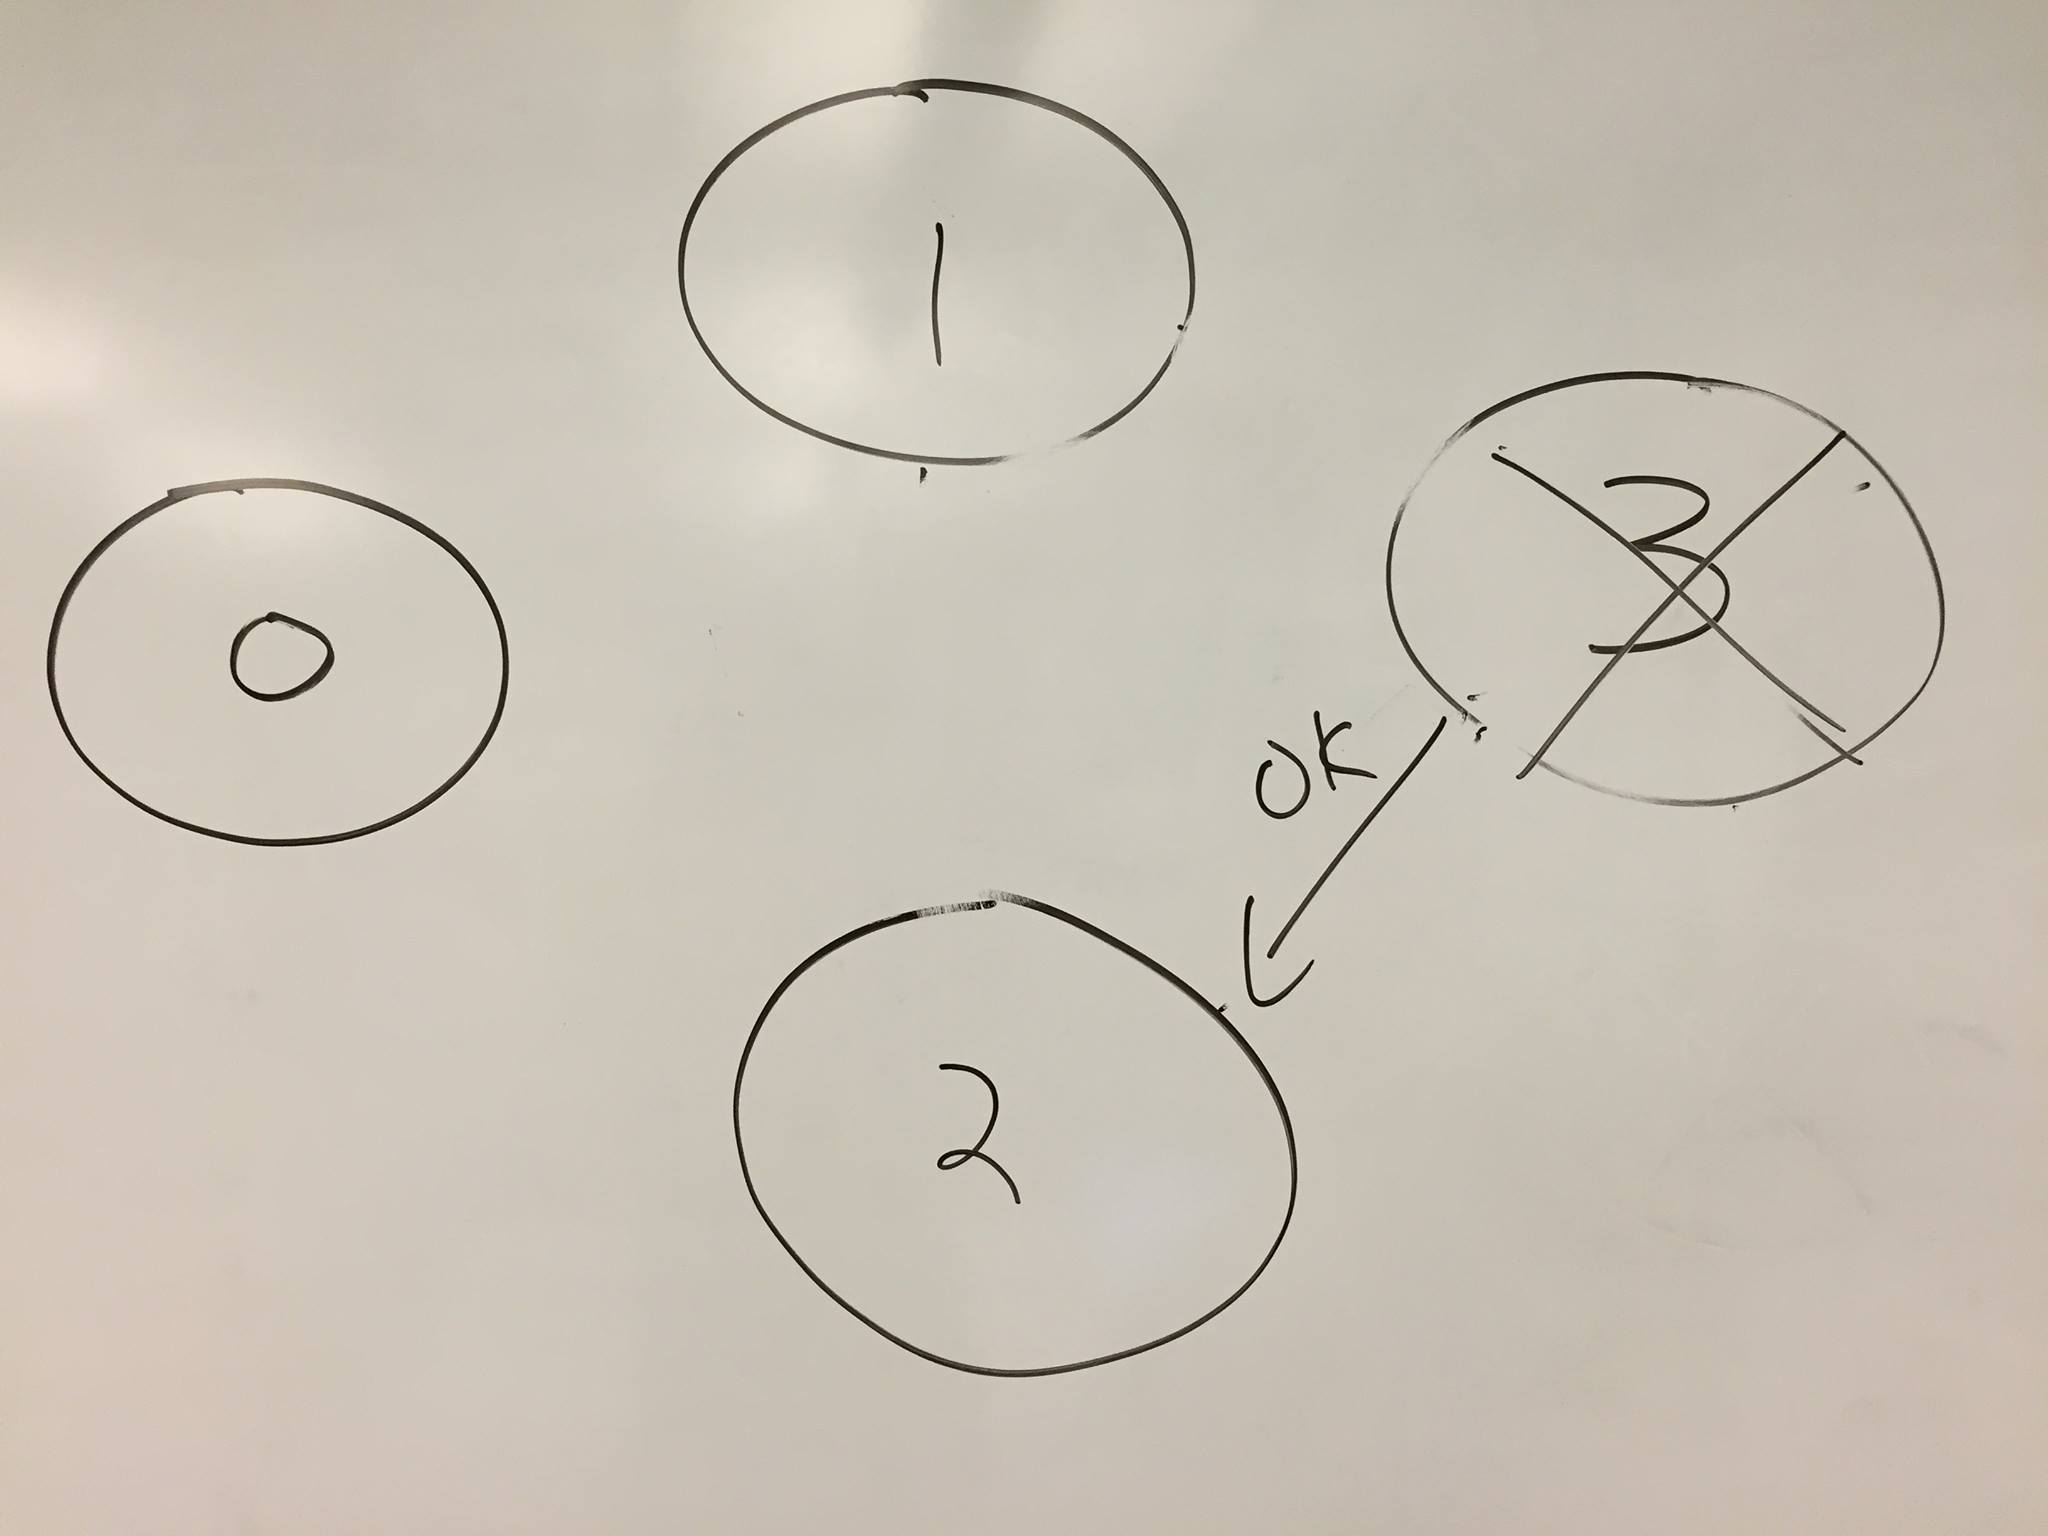
\includegraphics[scale=0.1]{nodes0}
\end{center}

Now the algorithm has undefined behaviour. Are nodes waiting for the leaders to finish deciding? Or are they waiting for a coordination message? Because there's uncertainty, the algorithm can't simply be restarted. This violates the progress property of the other nodes discovering the ID of the leader eventually. Without a coordination message broadcast, not everyone will know the ID of the winner (Progress Property 2).

\subsection*{b)}
\begin{itemize}
\item Suppose that after the algorithm completes, there will be more than one leader due to a crash.
\item Let's suppose we have to rerun the election because the previous leader crashed after an election occurred.
\item We have three steps in each iteration.
\item Case 1: If a node crashes after sending the election message, processes that originally sent the OK would begin their own election, and the algorithm continues, leading to a contradiction.
\item Case 2: If a process that sent an OK crashed and it was to become the leader, part (a) would follow, giving us less than two leaders - contradiction.
\item Case 3: If a process that sent an OK crashed and was not meant to become the new leader, then there would be no change to the algorithm - contradiction.
\end{itemize}
Conclusion: If we are only permitting one process crash at a time, there's no instance in which two processes could become the leader without the process with a higher ID eliminating the other lower ID leader.
\section{Consistency}
\subsection*{a) Sequentially Consistent}
T = < P1.W(x)a, P2.R(x)a, P3.R(x)a, P4.R(x)a, ...? >

We know it's not sequentially consistent because there's a discrepancy in the ordering of events for when  P1.W(x)c and P2.W(x)b occur. We see that P3 reads "c" first and then "b". This means that "c" needs to be written before "b", however, in P4, we see that "b" is read before "c", meaning that "c" needs to be written after "b". This creates a cycle in a DAG representation of the process ordering, proving that the execution is not sequentially consistent.

\begin{center}
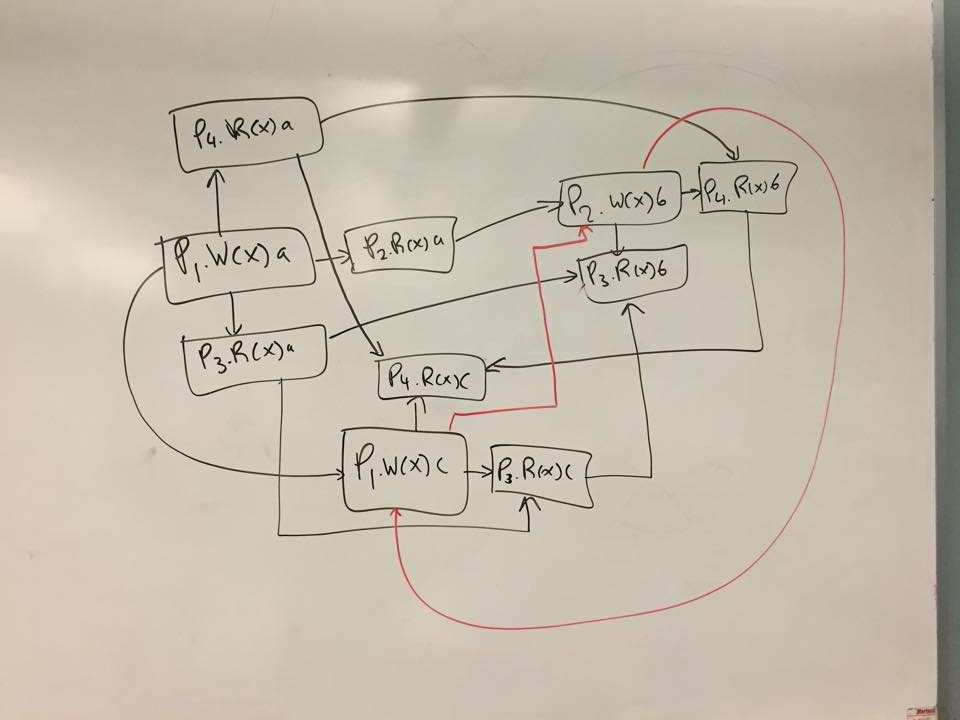
\includegraphics[scale=0.25]{sequential0}
\end{center}
\subsection*{b) Causally Consistent}
W(x)a happens first because P2, P3, and P4 read "a" first. P3 and P4 read "c" and "b" simultaneously, so they appear to have been written concurrently.

\begin{itemize}
\item T1 = < P1.W(x)a, P1.W(x)c >
\item T2 = < P1.W(x)a, P2.R(x)a, P2.W(x)b >
\item T3 = < P1.W(x)a, P3.R(x)a, P1.W(x)c, P3.R(x)c, P2.W(x)b, P3.R(x)b >
\item T4 = < P1.W(x)a, P4.R(x)a, P2.W(x)b, P4.R(x)b, P1.W(x)c, P4.R(x)c >
\end{itemize}

We have consistency in that the order in which "a" is read happens after it is written. Therefore, we have causal consistency on the operations up to the write of "b".
Despite P3 and P4 seeing the write for "c" and "b" in different orders, there's no restriction that prevents these two events from happening in either order or concurrently (i.e. P2.W(x)b needs to happen before some read on "a" in another process).

\section{NoSQL}
\subsection*{a)}
At $ \frac{2}{3} $ the speed of light, and with a distance of 3510km from Seattle to Atlanta, we have an approximate one-way delay of 17.6ms (time = $\frac{3510km}{2\cdot 10^5 km/s}$ ). This means that a round trip takes approximately 35ms. Therefore, we can successfully make requests between Atlanta and Seattle while still under our latency threshold.

Germany, however, is 8203km from Seattle. The distance here is over twice the distance of Seattle to Atlanta. Without doing the exact math, we know that twice the delay time is around 35ms, and doing that twice (Seattle to Frankfurt and back to Seattle) is going to take over 50ms.

Thus, this gives us two solutions. We can either use the "ONE" option or the "QUORUM" option since we can make queries to at least one other data center besides Seattle while still being under the latency threshold of 50ms.
\subsection*{b)}
Similar to part (a) we can use "ONE" or "QUORUM". The reasoning here is that we can use "QUORUM" to request two of the three remaining datacenters. We can also use "ONE" because internally, Cassandra makes requests to all data source replications. The difference functionally, between "ONE" and "QUORUM" is that Cassandra waits until it has all responses from the "QUORUM" before returning, but the "ONE" query will return the first response it gets, which could be from any of the data centers.
\subsection*{c)}
If N is 3 (because we have 3 data centers), then we want $N_R + N_W > N$. Taking this a step further, we also want $N_W + N_W > N$. This means that $N_W$ should be at least two. Then, to guarantee $N_R + N_W > N$, $N_R$ needs to be two as well.
We can use the "ALL" or the "QUORUM" consistency setting to achieve strong consistency. "ALL" will give us $N_W=3$ and $N_R=3$ and with "QUORUM" we can set our quorum size to be 3.
\subsection*{d)}
If the Atlanta data center goes down, the "QUORUM" option can't be used anymore. This is because we cannot afford to wait for responses from Frankfurt. We only get responses from the Seattle data center with queries less than 50ms of latency.
\end{document}